\documentclass[11pt,a4paper]{article}

\usepackage[utf8]{inputenc}
\usepackage[T1]{fontenc}
\usepackage{amsmath}
\usepackage{booktabs}
\usepackage{graphicx}
\usepackage{hyperref}
\usepackage{listings}
\usepackage{xcolor}
\usepackage[margin=1in]{geometry}

\definecolor{codegreen}{rgb}{0,0.6,0}
\definecolor{codegray}{rgb}{0.5,0.5,0.5}
\definecolor{codepurple}{rgb}{0.58,0,0.82}
\definecolor{backcolour}{rgb}{0.95,0.95,0.92}

\lstdefinestyle{mystyle}{
    backgroundcolor=\color{backcolour},
    commentstyle=\color{codegreen},
    keywordstyle=\color{magenta},
    numberstyle=\tiny\color{codegray},
    stringstyle=\color{codepurple},
    basicstyle=\ttfamily\footnotesize,
    breakatwhitespace=false,
    breaklines=true,
    captionpos=b,
    keepspaces=true,
    numbers=left,
    numbersep=5pt,
    showspaces=false,
    showstringspaces=false,
    showtabs=false,
    tabsize=2
}
\lstset{style=mystyle}

\title{Introducing Context-Fabric:\\[0.5em]
\large Scalable Corpus Analysis for the Agentic Era}
\author{Cody Kingham}
\date{Aug 2026}

\begin{document}

\maketitle

\begin{abstract}
For ten years, Text-Fabric (TF) has served as a powerful tool for corpus analysis, underlying 
an entire generation of linguistic and exegetical research. However, TF has always been burdened by two problems:
1) it is resource intensive, consuming large amounts of RAM; and 2) it requires knowledge of Python or
a query language to use it. These frictions have limited its usefulness to the philological community,
which is not known for its computational prowess!
Agentic AI, however, now makes it possible to solve the skill-gap. To maximize this opportunity,
TF must become light and agile, capable of running on resource-constrained systems, with the ability to scale to many corpora at once.
To address this, I introduce Context-Fabric (CF), a memory-efficient re-write of TF designed for the agentic era.
Using memory-mapped arrays to store the corpus graph, CF achieves up to a 92\% reduction in RAM consumption,
with as much as 5.3$\times$ more efficient scaling for multi-corpus loads. This is accomplished without sacrificing
search speeds, which are 3\% \textit{faster} overall, with direct feature look up improving 26\%. To take advantage
of this power, CF comes with an MCP server optimized for AI agents. This makes it possible to conduct complex,
high-level research without knowing a jot or tittle of Python.
\end{abstract}

\section{The Legacy of Text-Fabric}

In 1977, Eep Talstra founded the Werkgroep Informatica at the Vrije Universiteit Amsterdam
(today the Eep Talstra Centre for Bible and Computer, or ``ETCBC'') with the purpose of using
computers to analyze the Hebrew Bible.
Over the next fifty years, those efforts yielded a rich grammatical database
of Biblical Hebrew. For most of this period, the dataset was stored privately on the Werkgroep's
internal server.\footnote{
    It was also integrated into several paid software tools such as [†...CITE].
}
It was not until 2014 that Dirk Roorda, a research scientist on the [†?] project,
published the dataset online as an XML dump in Linguistic Annotation Framework (LAF) [†cite].
LAF models texts as graphs. The various linguistic units like clauses and phrases can be captured
as nodes with features, and their relations as edges [†cite https://link.springer.com/article/10.1007/s10579-014-9268-1].
Alongside the XML dump, Roorda published a Python package called LAF-Fabric, which could
walk the nodes and edges to query their features [†Roorda]. By choosing Python, Roorda 
simultaneously introduced Biblical Hebrew to the bourgeoning fields of Data Science
and Machine Learning, which had begun to widely adopt Python as the default scripting language.
One could, within the same program, collect statistics on a given grammatical pattern and
then apply complex statistical algorithms with tools like Numpy, Pandas, Scikit Learn, and others [†cite].
These new capabilities were soon picked up by enthusiasic researchers who leveraged them for a whole host
of studies. And they brought new emphasis on data-driven, reproducible results [† Synvar, Kalkan, Kingham, Naaijer, Jacobs, Erwich,
Glanz and team, etc. etc.].

In 2016, Roorda improved on the idea by releasing Text-Fabric (TF) [†Roorda]. TF
dramatically reduced the disk storage needed for the graph data by replacing in-line XML
with a stand-off plain-text format, the \texttt{.tf} file. It made the graph data modular so that
each \texttt{.tf} file contributed a single node feature or edge relationship. If one only wanted to analyze
verb tense, for instance, he could choose to load only the \texttt{vt} feature.\footnote{
    Plus some required node type and slot edge relations.
}
The \texttt{.tf} format is a single column of data, with each row indexed by its node identifier.
This strips away the syntactic overhead required by the XML format, reducing disk space and load times.
Roorda envisioned that this new nimble format, along with a host of user-friendly visualization tools,
would catalyze a new category of scholar, the ``programming theologian''.

The vision of the computational theologian was certainly ambitious, and it dovetailed well with
the ETCBC's heritage; but its success was always hampered by one minor problem: learning to code
is hard. And that difficulty was compounded by the right-brained tendencies of humanities students
who were more comfortable writing exegetical summaries than loops and conditions. That is not
to say the idea failed. Indeed, the study of syntax is closely aligned to left-brained tendencies,
and many enterprising scholars followed the Roordian path. But the dream's true fulfillment---of a humanities
field radically transformed by a \textit{scientific} approach---simply could not be realized given the
skill gap.

Such was the state of things until 2022, when OpenAI announced on Twitter the release of a new
public demo of its Large Language Model (LLM), ChatGPT [†cite]. This is the ``AD'' moment that will,
most likely, come to separate the eras of manually-written and machine-generated code.
The first beachhead was autocomplete, which could generate entire functions, fit for purpose, on the fly.
Yet, most code continued to be written by hand within closely-supervised IDEs. For many engineers, the
true moment of surrender came around December 2025, when Anthropic released its \texttt{Opus 4.5} model alongside
its \textit{Claude Code} tool. Here was a tool which could reliably generate entire software packages in one go,
complete with tests and documentation. Since then, the trend towards agentic-authored code has sharply accelerated
with the encouragement of additional models and tools (e.g.~Codex, Grok Build, open source weights) and competitive
pressure.

The AI revolution now makes it possible to fully realize Roorda's vision, closing the skill gap that made Text-Fabric
inaccessible for most. To maximize this opportunity, several transformations to Text-Fabric are required.
First, corpus search must become \textit{deployable} to a production environment.
This means the ability to serve search from a persistent web server for
thousands of requests at a time. This will enable AI agents to search remotely from any sandbox environment
they happen to be running in. This requires a change to the way TF accesses the text graph. The current
approach loads all nodes and edges into RAM, consuming a significant amount of memory. In production,
especially under high loads, this is untennable. Memory mapping offers an alternative where graph data can
be stored on disk and accessed only when needed. This method is already used
by a number of performance-sensitive machine learning tools like Pytorch and Tensorflow [†cite].
Second, Text-Fabric must be enhanced to automatically build and return corpora descriptions that can
be consumed by AI agents. These descriptions are crucial for agents to know what nodes, edges, and features
are available for searching. Ideally, these descriptions would be completely corpus-agnostic so that they
work out-of-the-box with pre-existing corpora. Additionally, Text-Fabric should return a syntax guide
for running TF queries. The guide should be optimized for progressive discovery, so that agents can drill down
to the specific patterns they require while ignoring the rest.

These requirements reach deep into Text-Fabric's data model and radically transform what is possible.
For this reason, and in the spirit of TF's previous evolution from LAF-Fabric, I have chosen to rename
and re-release this tool as Context-Fabric (CF). The name is a nod to the critical role of context engineering
in agentic applications. The package is released under the same MIT license under a new shared organization,
open for pull requests. CF implements a memory mapped data model using Numpy's \texttt{memmap} function with
\texttt{.npy} files, replacing TF's in-memory Python dictionaries. Several optimizations are applied to ensure
that the latency penalty of disk streaming is compensated for. In the end, CF pulls slightly ahead of TF for
search speeds. Meanwhile, RAM usage drops sharply, and load times go from several seconds to nearly isntantaneous.
For corpus description and search syntax, CF provides a set of API methods which automatically analyze and sample
the text graph, giving the agent a full map along with illustrative examples. This works even with various transcription
formats. The search guide is implemented with different ``menus'', allowing the agent to drill down to specific
sub-topics as needed. These methods are wired to an optional MCP server (Model Context Protocol) which ships alongside
CF.

\section{Migrating Text-Fabric's Data Model}

\subsection{The Text as Graph}

Text-Fabric's data model is the ``text as graph''. A corpus is conceived of
as a collection of nodes (objects of interest), which may have edges (relationships). Different
types of attributes, or features, can be stored on nodes and edges. Figure †TODO illustrates the
organization. All nodes in the graph have an object type feature, \texttt{otype}. The only obligatory
\texttt{otype} is the slot, which defines the atomic units (e.g.~words, letters) which comprise the text.
There is a corresponding, obligatory edge value from slots to other nodes, which is called \texttt{oslots}.
This edge defines the containment relationship between a given node and its slots. For example, node
\texttt{503201} in Figure~[†TODO] \textit{contains} slots \texttt{1} and \texttt{2}, and therefore has
an \texttt{oslots} edge extending to both nodes. Containment between non-slot nodes (e.g. phrase in clause)
is automatically inferred from slot intersection, and need not be encoded separately.\footnote{
    The arrows in the figure, in this sense, do not represent directly represent edge relations.
}

% INSERT figure: file:///Users/cody/github/context-fabric/context-fabric/site/public/docs/images/containment-hierarchy.svg

Descriptive attributes, or features, can be stored on both nodes and edges. For example, the first phrase
node can have a \texttt{typ} feature with a value of \texttt{PP}, for ``prepositional phrase type''.
Likewise, embedded clauses may have an edge to another clause with the name of \texttt{rela} and
a value of \texttt{Attr} for ``attributive clause''. Text-Fabric itself is agnostic about which kinds
of nodes and edges a corpus encodes, with the exception of the aforementioned obligatory types.
The text-as-graph model is powerful in its flexibility and expressiveness. For this reason, it is
desirable to retain it.

\subsection{TF's Python Dictionaries}

In Python, dictionaries are container classes that provide interactions with a hash table.
In plain terms, they efficiently route a given key to a given value, and are used for storing 
data as key-value pairs. Thus, given a dictionary named \texttt{oslots},
one can use a node number to very quickly look up the corresponding
slot values. This architecture underlies Text-Fabric's corpus loading algorithm, which populates
a collection of dictionaries into memory. The approach has the advantage of being very fast, with
the tradeoff of massive memory consumption. Large corpora can consume gigabytes. The ETCBC's 
\texttt{.tf} Hebrew Bible, for example, takes up to [†TODO] GB of RAM when fully unfolded. 
The in-memory dictionary based storage is the critical component that needs to be changed to make
loading and usage efficient.

% TODO: insert illustrative code block here

\subsection{Adapting to Memory Mapped Arrays}

An alternative way to store key-value pairs is with linked arrays. 

Memory-mapped I/O (\texttt{mmap}) maps file contents directly into a process's virtual address space \cite{wikipediammap}. Rather than explicitly reading data into buffers, the program accesses file contents through pointers, and the OS transparently pages data in and out as needed.

NumPy's \texttt{memmap} function provides a Python interface for memory-mapping array data \cite{numpymemmap}. Context-Fabric stores all corpus data as \texttt{.npy} files and loads them with \texttt{mmap\_mode='r'} (read-only), enabling safe multi-process sharing.


The challenge is converting Text-Fabric's Python-native data structures to memory-mappable formats while preserving the same Python interface that existing code expects.

\subsubsection{Dense Arrays for Node Features}

Node features with single values per node map directly to numpy arrays. The storage format depends on the feature's value type:

\textbf{Integer features} (verse numbers, word positions) store values directly in appropriately-sized dtypes (\texttt{uint8}, \texttt{uint16}, \texttt{uint32}).

\textbf{Categorical features} with small value sets use index encoding. The node type feature (\texttt{otype}), for example, maps each node to one of a handful of type names (``word'', ``verse'', ``chapter'', etc.). Since corpora typically have fewer than 256 node types, these indices fit in a \texttt{uint8} array:

\begin{lstlisting}[language=Python, caption=Categorical feature storage]
# Type names: ["word", "verse", "chapter", ...]
# otype[node_id] = index into type_names
otype = np.array([0, 0, 0, ..., 1, 1, 2, ...], dtype=np.uint8)

# Lookup: O(1)
node_type = type_names[otype[node_id]]  # -> "word"
\end{lstlisting}

This is conceptually similar to the string pool pattern (described next), but optimized for small, fixed value sets.

\subsubsection{String Pools for Text Features}

String-valued features (glosses, lexemes, morphological tags) present two challenges. First, Python strings cannot be memory-mapped directly. Second, not every node has a value for every feature---Text-Fabric represents these as \texttt{None}, but NumPy integer arrays have no native missing-value representation (unlike floats, which have \texttt{NaN}).\footnote{While float arrays could use \texttt{NaN} for missing values, storing indices as floats wastes memory (float64 is 8 bytes vs.\ uint16's 2 bytes for most features), requires type conversion on every lookup, and is semantically misleading since indices are inherently integers.}

Context-Fabric addresses both with a string pool pattern. Unique strings are stored once in an array, with a separate index array mapping each node to its string's position. For missing values, we reserve a sentinel index: \texttt{0xFFFFFFFF} (the maximum \texttt{uint32} value, $2^{32}-1$). This value cannot be a valid index---it would require over 4 billion unique strings---so encountering it unambiguously signals ``no value.'' This preserves the distinction between an empty string (a valid value at some index) and a truly absent value.

\begin{lstlisting}[language=Python, caption=String pool structure]
MISSING = 0xFFFFFFFF  # Sentinel for "no value" (max uint32)

# Feature "gloss" for 5 nodes: ["king", "the", "king", None, "house"]
strings = np.array(["king", "the", "house"], dtype=object)  # Unique values
indices = np.array([0, 1, 0, MISSING, 2], dtype=np.uint32)  # Per-node index

def lookup(node):
    idx = indices[node]
    return None if idx == MISSING else strings[idx]

lookup(2)  # -> "king"
lookup(3)  # -> None (missing value)
\end{lstlisting}

The \texttt{indices} array is memory-mapped (\texttt{uint32}, one entry per node). The \texttt{strings} array is small---most features have far fewer unique values than nodes---and loads into memory. For BHSA's \texttt{gloss} feature, 426,590 words map to roughly 9,000 unique glosses.

\subsubsection{Compressed Sparse Row Format}

Some corpus data involves variable-length sequences. Consider \texttt{oslots}, which maps each non-slot node to the word positions it contains: a 3-word phrase contains slots \texttt{[5, 6, 7]}, while a 20-word verse contains \texttt{[100, 101, ..., 119]}. In Python, Text-Fabric stores this as a tuple of tuples---but Python tuples are pointers to objects scattered across memory, which cannot be memory-mapped.

Context-Fabric solves this with Compressed Sparse Row (CSR) format: concatenate all sequences into one flat \texttt{data} array, and use a separate \texttt{indptr} (index pointer) array to record where each sequence begins and ends:

\begin{lstlisting}[language=Python, caption=CSR format for oslots]
# oslots for 3 nodes: phrase contains [5,6,7], clause contains [5,6,7,8], verse contains [5..12]
# Concatenate all slots into one array:
data   = [5, 6, 7, 5, 6, 7, 8, 5, 6, 7, 8, 9, 10, 11, 12]

# Record boundaries (one entry per node, plus final endpoint):
indptr = [0, 3, 7, 15]

# Lookup: node i's slots are data[indptr[i] : indptr[i+1]]
phrase_slots = data[0:3]   # -> [5, 6, 7]
clause_slots = data[3:7]   # -> [5, 6, 7, 8]
verse_slots  = data[7:15]  # -> [5, 6, 7, 8, 9, 10, 11, 12]
\end{lstlisting}

Both arrays are flat numpy arrays that can be memory-mapped. The \texttt{indptr} array has length $N+1$ (one boundary per node, plus the final endpoint). Empty sequences cost nothing: when \texttt{indptr[i] == indptr[i+1]}, the slice is empty.

For edge features with associated values (e.g., linguistic dependency weights), \texttt{CSRArrayWithValues} adds a parallel values array:

\begin{lstlisting}[language=Python, caption=CSR with values]
# Edge feature "distance": node 0 -> {10: 100, 20: 200}, node 1 -> {}, node 2 -> {30: 300}
# (node 0 connects to nodes 10 and 20 with distances 100 and 200)
indptr  = [0, 2, 2, 3]      # Boundaries
indices = [10, 20, 30]      # Target nodes
values  = [100, 200, 300]   # Associated values (e.g., distances)

def get_edges(node):
    start, end = indptr[node], indptr[node + 1]
    return indices[start:end], values[start:end]

get_edges(0)  # -> ([10, 20], [100, 200])  node 0's targets and distances
get_edges(1)  # -> ([], [])                node 1 has no edges
get_edges(2)  # -> ([30], [300])           node 2 connects to 30
\end{lstlisting}

All arrays use \texttt{uint32} dtype and load via \texttt{mmap\_mode='r'} (read-only), enabling safe multi-process sharing without copy-on-write overhead.

\subsubsection{The \texttt{.cfm} Format}

Context-Fabric's compiled format (\texttt{.cfm}) organizes data into a directory structure:

\begin{lstlisting}[language=bash, caption=.cfm directory structure]
corpus/                   # Corpus directory (e.g., bhsa/)
  .cfm/                   # Hidden compiled-format subdirectory
    meta.json             # Corpus metadata
    warp/
      otype.npy           # Node types (uint8)
      oslots_indptr.npy   # CSR boundaries
      oslots_data.npy     # CSR slot data
    computed/
      order.npy           # Traversal order
      rank.npy            # Node ranks
      levup_indptr.npy    # Embedder CSR
      levup_data.npy
    features/
      sp.npy              # Part of speech (dense)
      gloss_idx.npy       # String pool indices
      gloss_strings.npy   # Unique strings
    edges/
      mother_indptr.npy   # Edge CSR
      mother_data.npy
\end{lstlisting}

\subsubsection{Optimizing Search Performance}

The problem: paging into on-disk storage is slow. To compensate, Context-Fabric must
improve on Text-Fabric's search algorithm. As it turns out, memory-mapping with vectors
also makes possible vectorized lookup, with major speed gains on certain operations.
In TF search, feature-based lookup is linear (O(n) time complexity):

\begin{lstlisting}[language=Python, caption=Per-node iteration (original)]
for node in candidate_nodes:
    if feature.value(node) == target_value:
        result.add(node)
\end{lstlisting}

Instead of linear search we use vectorized lookup, which is O(1):

\begin{lstlisting}[language=Python, caption=Vectorized filtering]
node_array = np.array(list(candidate_nodes))
values = feature_data[node_array - 1]
mask = values == target_index
result = set(node_array[mask])
\end{lstlisting}

The vectorized strategy yields nearly an order of magnitude lower latency (8.2$\times$),
translating to 26\% faster feature lookups in real-world benchmarks.

However, tests continued to show significant slowdowns on searches involving containment of node types.
For example, looking for a phrase which occurs within a particular clause resulted in substantially increased
search latency, due to page faults while accessing the disk. Thus, the decision was made to include an optional
in-memory load for pre-calculated node containment features (i.e.~LevUp and LevDown [†check spelling] from Text-Fabric).
For the BHSA, this costs \texttt{100 MB} but yields a 1.7$\times$ speedup for containment search. This offsets
the page-fault penalty and brings CF to parity with TF for containment search.

\subsection{Benchmarking and Results}

To quantify Context-Fabric's improvements, I conducted systematic benchmarks across memory efficiency,
multi-corpus scaling, and query latency. This section describes the methodology; results follow in
Section~\ref{sec:results}.

All benchmarks were conducted on:

\begin{itemize}
    \item \textbf{Hardware}: Apple M1 Pro, 8 cores, 32 GB RAM, NVMe SSD
    \item \textbf{OS}: macOS Darwin 24.5.0 (arm64)
    \item \textbf{Python}: 3.13.11
    \item \textbf{NumPy}: 2.4.0
    \item \textbf{Text-Fabric}: 13.0.19
    \item \textbf{Context-Fabric}: 0.5.0
\end{itemize}

Production Linux deployments may show different absolute numbers but similar relative performance characteristics.

\subsection{Test Corpora}

Benchmarks span 10 corpora representing three orders of magnitude in size, from 1.6 MB to 1.1 GB. Table~\ref{tab:test_corpora} lists the corpora in order of increasing size.

\begin{table}[htbp]
\centering
\caption{Test corpora used in benchmarks, ordered by TF cache size.}
\label{tab:test_corpora}
\begin{tabular}{llr}
\toprule
\textbf{Corpus} & \textbf{Description} & \textbf{TF Cache Size} \\
\midrule
CUC \cite{cuc} & Copenhagen Ugaritic Corpus & 1.6 MB \\
Tischendorf \cite{tischendorf} & Tischendorf 8th Edition Greek NT & 34 MB \\
SyrNT \cite{syrnt} & Syriac New Testament & 52 MB \\
Peshitta \cite{peshitta} & Syriac Old Testament & 55 MB \\
Quran \cite{quran} & Quranic Arabic Corpus & 73 MB \\
SP \cite{sp} & Samaritan Pentateuch & 147 MB \\
LXX \cite{lxx} & Septuagint & 268 MB \\
N1904 \cite{n1904} & Nestle 1904 Greek NT & 319 MB \\
DSS \cite{dss} & Dead Sea Scrolls & 936 MB \\
BHSA \cite{bhsa} & Biblia Hebraica (ETCBC) & 1.1 GB \\
\bottomrule
\end{tabular}
\end{table}

This diversity enables analysis of how memory efficiency scales with corpus size. The BHSA (largest corpus) provides richly annotated linguistic data for the Hebrew Bible, containing 1,446,831 total nodes, 426,590 word-level nodes, 13 node types, 109 node features, and 6 edge features.

% \subsection{Measurement Protocol}

Each benchmark configuration runs 10 independent measurement runs following 2 warmup runs (excluded from statistics). Measurements use subprocess isolation via \texttt{multiprocessing.spawn} to ensure clean memory state, with explicit \texttt{gc.collect()} before measurement.\footnote{Load time refers to the time from initiating corpus load to having a usable API handle, measured using Python's \texttt{time.perf\_counter()}.}

% \subsection{Memory Metrics}

Operating systems provide several metrics for quantifying process memory \cite{beyer2019reliable}. \textbf{Resident Set Size (RSS)} measures physical memory pages mapped to a process, including private allocations and shared pages \cite{wikipediarss}. \textbf{Unique Set Size (USS)} counts only pages unique to a process, excluding shared memory. \textbf{Proportional Set Size (PSS)} divides shared pages proportionally among processes \cite{baeldunglinuxmem}.

We use RSS for all measurements. While RSS double-counts shared pages in multi-process scenarios, this ``worst case'' view provides transparency: the numbers represent actual memory pressure on the system. USS would dramatically undercount Context-Fabric's memory-mapped data (potentially showing near-zero for file-backed pages), while PSS is unavailable on macOS and fluctuates as processes start and stop.

% \subsection{Measurement Isolation}

To ensure accurate measurements uncontaminated by prior allocations, each scenario runs in an isolated subprocess:

\begin{lstlisting}[language=Python, caption=Subprocess isolation pattern]
def _measure_cache_load(source: str, result_queue):
    """Runs in a clean spawned subprocess."""
    # Load corpus from cache
    fabric = Fabric(locations=source)
    api = fabric.load()

    # Measure total RSS after loading
    gc.collect()
    total_rss = psutil.Process().memory_info().rss
    result_queue.put(total_rss)

# Main process spawns clean subprocess
ctx = multiprocessing.get_context('spawn')
p = ctx.Process(target=_measure_cache_load, args=(source, queue))
p.start()
\end{lstlisting}

This pattern ensures:
\begin{enumerate}
    \item No residual memory from compilation or prior measurements
    \item Consistent baseline across Text-Fabric and Context-Fabric
    \item Reproducible results across runs
\end{enumerate}

\subsection{Deployment Scenarios}

We evaluate three scenarios representing common deployment patterns:

\subsubsection{Single Process}

A single Python process loads the corpus from cache and serves requests. This represents interactive research use or single-threaded batch processing.

\textbf{Measurement}: Total RSS of subprocess after cache load.

\subsubsection{Spawn Mode (4 Workers)}

Four independent worker processes, each loading the corpus from scratch. This simulates \texttt{multiprocessing} with \texttt{spawn} context---the default on macOS and the only option on Windows.\footnote{Windows lacks a \texttt{fork()} system call entirely. On macOS, \texttt{fork()} is available but Python 3.8+ defaults to \texttt{spawn} because forking processes that use certain Apple frameworks (Cocoa, Core Foundation) can cause crashes. Production deployments can explicitly use \texttt{fork} via \texttt{multiprocessing.get\_context('fork')} when the application avoids these frameworks.}

\textbf{Measurement}: Sum of RSS across all 4 worker processes.

\subsubsection{Fork Mode (4 Workers)}

A main process pre-loads the corpus, then forks 4 worker processes. Workers inherit the loaded corpus via copy-on-write semantics. This simulates production deployments like \texttt{gunicorn --preload}. Fork mode is the default on Linux systems in Python 3.13 and earlier.\footnote{Python 3.14 (October 2025) changed the default to \texttt{forkserver} on Linux. Applications requiring fork must explicitly request it via \texttt{multiprocessing.get\_context('fork')}.}

\textbf{Measurement}: Main process RSS + sum of worker RSS.

Note: For fork mode, summing RSS across processes may double-count shared copy-on-write pages. This is intentional---we report the ``worst case'' RSS sum rather than attempting to deduplicate shared pages, which would require USS and reintroduce the transparency issues discussed above.

\subsection{Query Performance Methodology}

Query latency was measured using 100 curated search templates on the BHSA corpus, categorized into four types:

\begin{itemize}
    \item \textbf{Lexical queries} (30): Feature-based filtering (e.g., find all verbs, filter by part of speech)
    \item \textbf{Structural queries} (30): Pattern matching across hierarchical structures
    \item \textbf{Quantified queries} (20): Queries using quantifiers (\texttt{<}, \texttt{>}, \texttt{..})
    \item \textbf{Complex queries} (20): Multi-constraint queries combining relations and features
\end{itemize}

Each query executes 50 times (5 runs $\times$ 10 iterations per run), with warmup iterations excluded. We report mean latency, standard deviation, and 95\% confidence intervals.

\subsection{Statistical Analysis}

Results report mean values with 95\% confidence intervals computed from 10 measurement runs per configuration. Linear regression models characterize scaling behavior, reporting slope, intercept, and $R^2$ values. Memory reduction percentages are computed as $(M_{\text{TF}} - M_{\text{CF}}) / M_{\text{TF}} \times 100$.

\section{Results}
\label{sec:results}

The benchmark suite covers three dimensions of performance: memory efficiency across 10 diverse corpora, multi-corpus scaling behavior, and query latency across 100 representative queries. This section presents each dimension in turn.

\subsection{Memory Efficiency Across Corpora}
\label{sec:results-memory}

Table~\ref{tab:memory_multicorpus} presents memory consumption for single-process corpus loading across all 10 benchmarked corpora, ordered by size. The results demonstrate a clear relationship between corpus size and memory reduction: smaller corpora exhibit modest reductions (20\% for CUC at 1.6 MB), while larger corpora show dramatic improvements (92\% for BHSA at 1.1 GB). The average memory reduction across all corpora is 65\% ($\pm$21\%).

\begin{table}[htbp]
\centering
\caption{Memory efficiency comparison across 10 corpora in single-process mode. Corpora ordered by TF memory footprint. Load time speedup calculated as TF load time / CF load time.}
\label{tab:memory_multicorpus}
\begin{tabular}{lrrrrr}
\toprule
\textbf{Corpus} & \textbf{TF (MB)} & \textbf{CF (MB)} & \textbf{Reduction} & \textbf{Load Speedup} \\
\midrule
CUC            &    164 &    131 &  20\% & 0.52$\times$ \\
Tischendorf    &    304 &    146 &  52\% & 1.62$\times$ \\
Quran          &    401 &    187 &  54\% & 1.29$\times$ \\
Peshitta       &    404 &    173 &  57\% & 0.96$\times$ \\
Syrnt          &    515 &    145 &  72\% & 3.08$\times$ \\
SP             &    644 &    174 &  73\% & 4.25$\times$ \\
LXX            &  1,395 &    388 &  72\% & 1.25$\times$ \\
N1904          &  1,566 &    411 &  74\% & 2.41$\times$ \\
DSS            &  3,233 &    337 &  90\% & 6.24$\times$ \\
BHSA           &  6,292 &    524 &  92\% & 12.91$\times$ \\
\midrule
\textbf{Mean}  &  1,492 &    262 &  65\% & 3.45$\times$ \\
\bottomrule
\end{tabular}
\end{table}

The distribution shows that memory reduction scales approximately with corpus size. For the smallest corpus (CUC), Context-Fabric achieves only 20\% reduction because the baseline overhead of Python's runtime and library imports dominates the measurement. For the largest corpus (BHSA), reduction reaches 92\%---a 12-fold decrease in memory footprint. Figure~\ref{fig:memory_multicorpus} visualizes this relationship.

\begin{figure}[htbp]
\centering
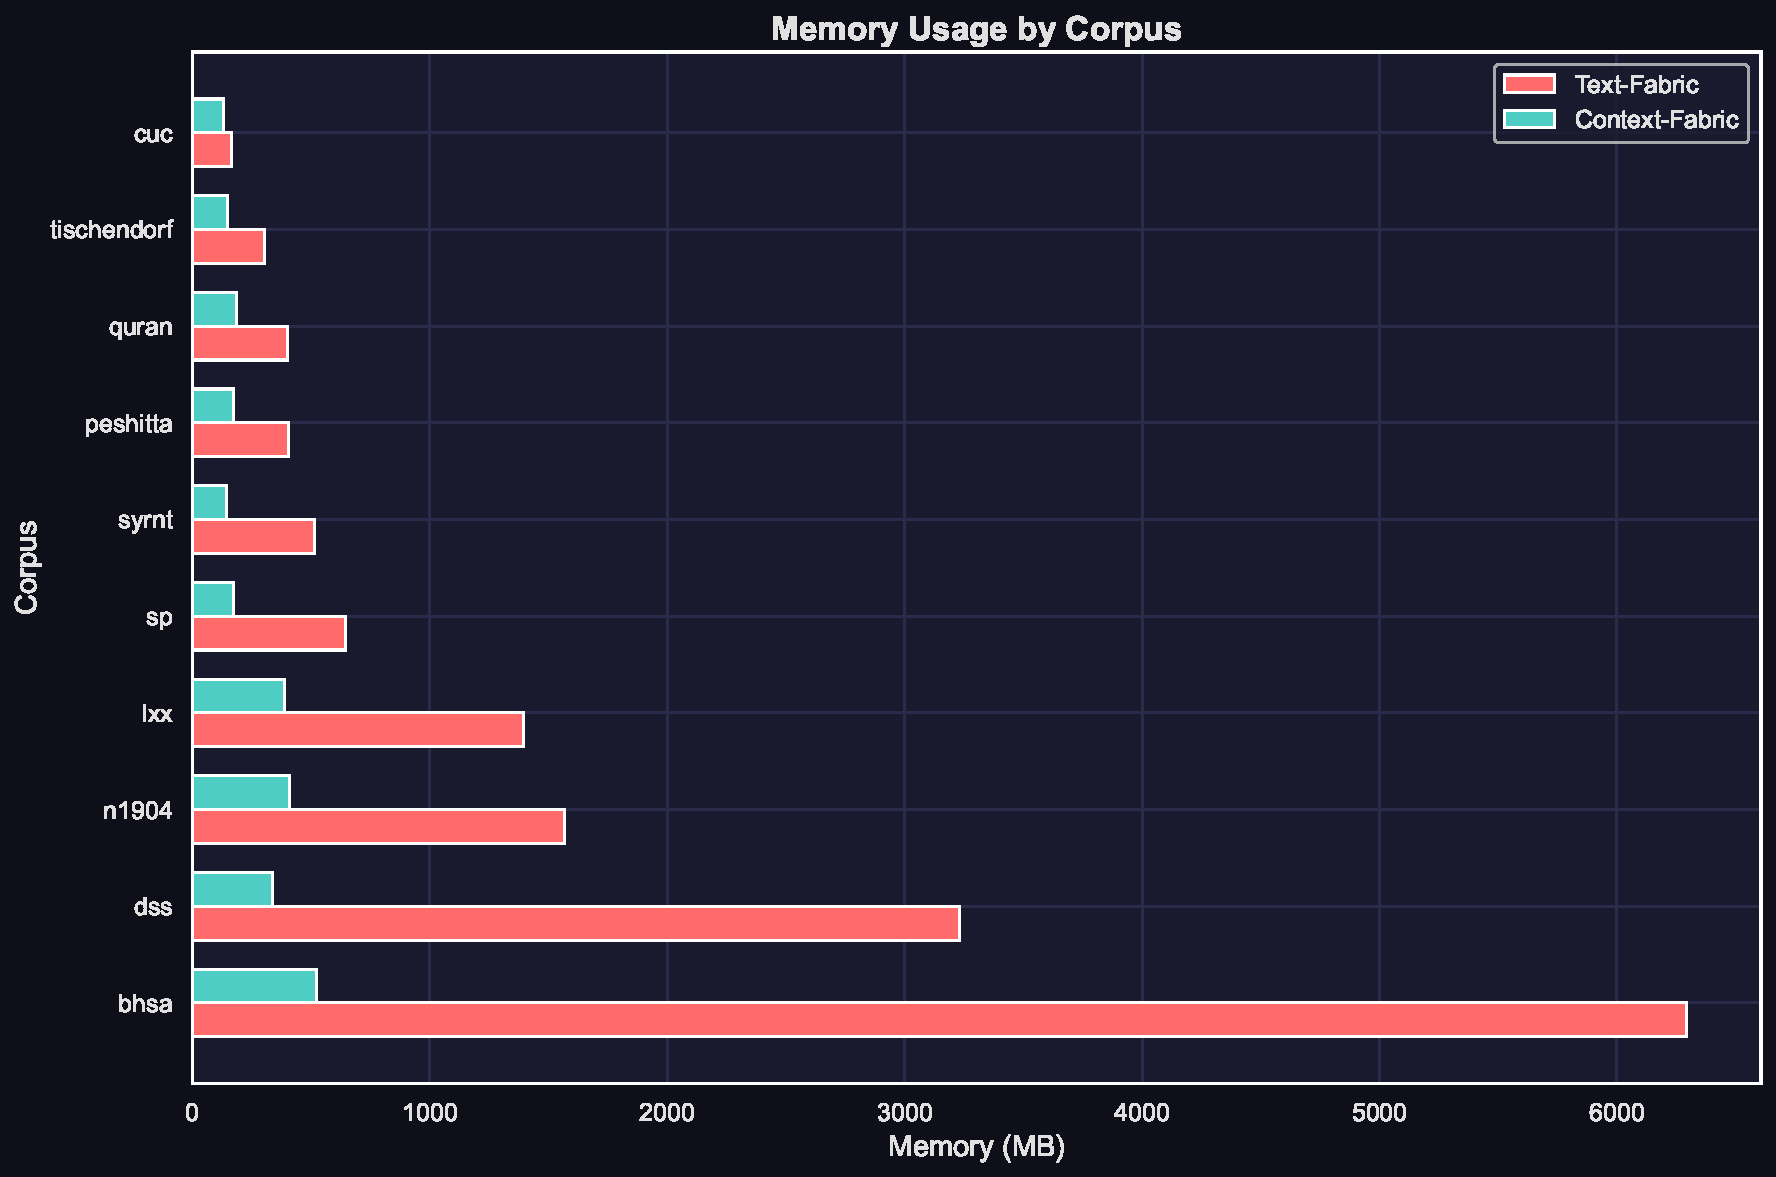
\includegraphics[width=0.9\textwidth]{fig_memory_multicorpus.pdf}
\caption{Memory consumption comparison across 10 corpora, sorted by Text-Fabric memory footprint. Error bars show 95\% confidence intervals over 10 measurement runs.}
\label{fig:memory_multicorpus}
\end{figure}

The load time results exhibit more variance. Context-Fabric achieves substantial speedups for larger corpora (12.9$\times$ for BHSA, 6.2$\times$ for DSS), but shows neutral or slightly slower load times for smaller corpora. This pattern reflects a fundamental tradeoff: Context-Fabric's memory-mapped architecture incurs fixed initialization costs that dominate for small datasets but amortize effectively as corpus size grows.

\subsection{Multi-Corpus Scaling Analysis}
\label{sec:results-scaling}

A key advantage of memory-mapped architecture emerges when loading multiple corpora simultaneously---a common requirement for comparative linguistic analysis. Table~\ref{tab:progressive} summarizes the progressive loading results, where corpora are loaded incrementally in order of increasing size.

\begin{table}[htbp]
\centering
\caption{Memory consumption during progressive multi-corpus loading. Values represent mean total RSS (MB) across 5 runs after loading the specified number of corpora.}
\label{tab:progressive}
\begin{tabular}{crrrr}
\toprule
\textbf{Corpora Loaded} & \textbf{TF (MB)} & \textbf{CF (MB)} & \textbf{Reduction} & \textbf{Ratio} \\
\midrule
1 (CUC)         &    163 &    130 &  20\% & 1.3$\times$ \\
2 (+Tischendorf) &    306 &    146 &  52\% & 2.1$\times$ \\
3 (+Syrnt)      &    641 &    161 &  75\% & 4.0$\times$ \\
4 (+Peshitta)   &    866 &    204 &  76\% & 4.2$\times$ \\
5 (+Quran)      &  1,070 &    259 &  76\% & 4.1$\times$ \\
6 (+SP)         &  1,531 &    300 &  80\% & 5.1$\times$ \\
7 (+LXX)        &  2,717 &    551 &  80\% & 4.9$\times$ \\
8 (+N1904)      &  4,044 &    791 &  80\% & 5.1$\times$ \\
9 (+DSS)        &  6,088 &    968 &  84\% & 6.3$\times$ \\
10 (+BHSA)      &  5,529 &  1,348 &  76\% & 4.1$\times$ \\
\bottomrule
\end{tabular}
\end{table}

Note that the step 10 TF mean (5,529 MB) is anomalously lower than step 9 (6,088 MB). This probably results from Python's garbage collector triggering non-deterministically at high memory: two of five runs showed $\sim$1,750 MB drops mid-measurement, while others showed expected growth. The resulting variance ($\pm$949 MB for TF vs. $\pm$7 MB for CF) reflects this unpredictability rather than true memory reduction.

Polynomial regression reveals distinct scaling characteristics. Both implementations fit quadratic models better than linear ($R^2$ improves from $\sim$0.83 to $\sim$0.98), but the critical difference is the quadratic coefficient: TF grows as 126$n^2$ MB while CF grows as only 19$n^2$---a 6.5$\times$ difference in compounding overhead. For practical corpus counts ($\leq$20), CF's weak quadratic term is negligible; TF's is not. The linear approximation (TF: 677 MB/corpus, CF: 127 MB/corpus) captures first-order behavior but understates TF's compounding overhead at scale.

\begin{figure}[htbp]
\centering
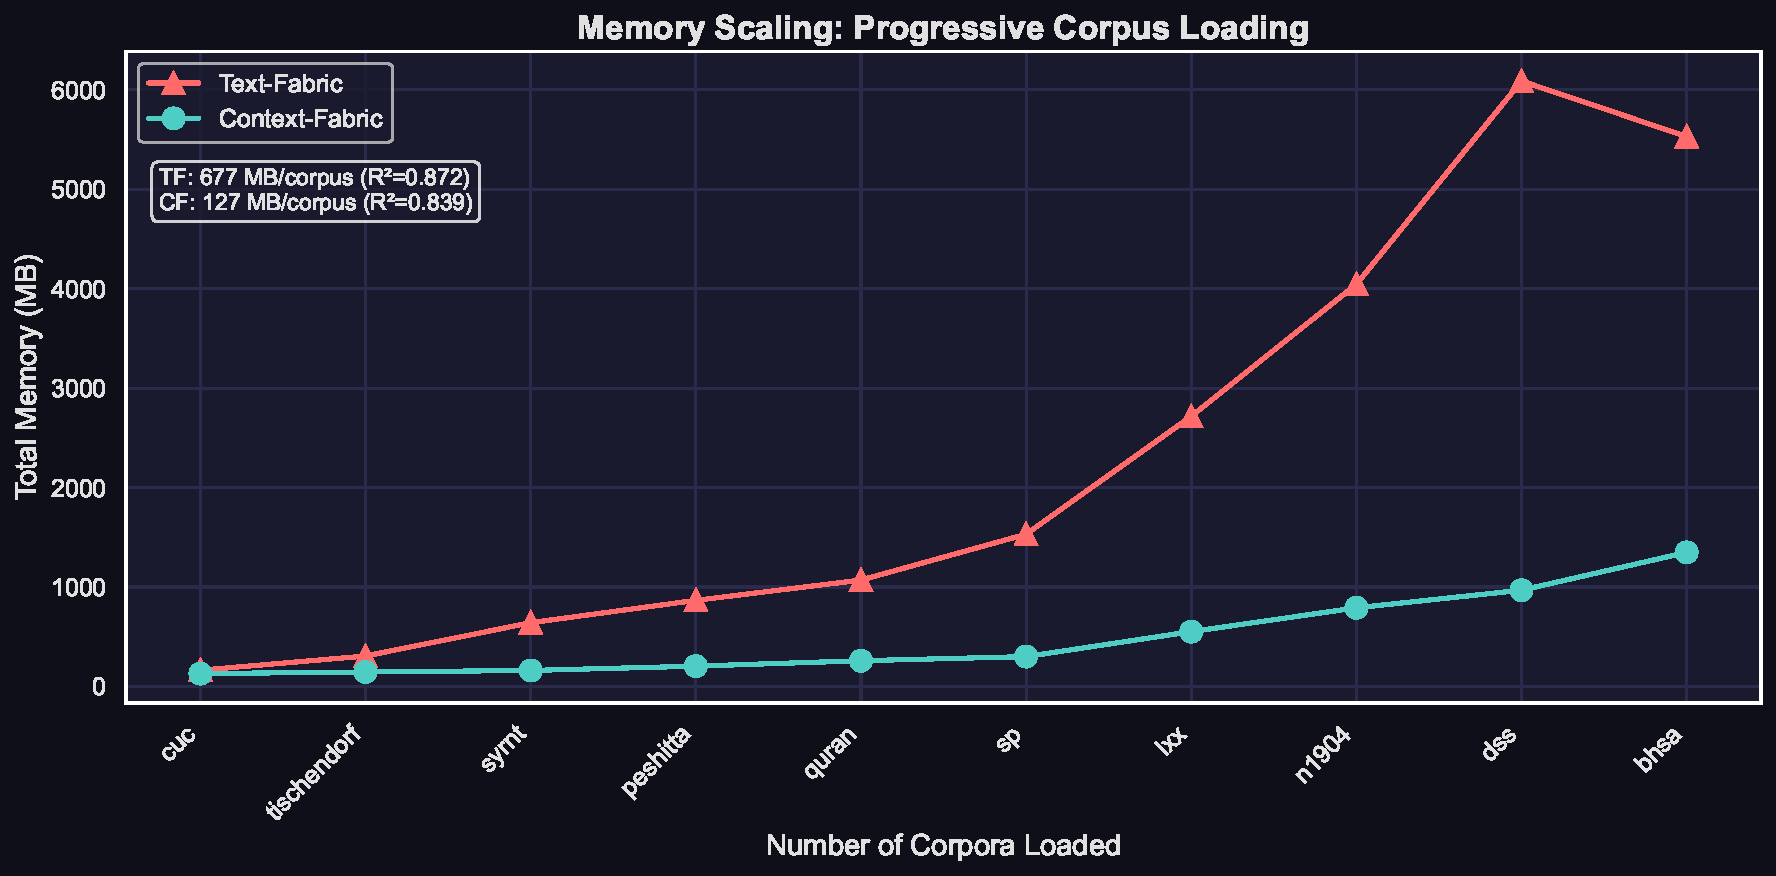
\includegraphics[width=0.9\textwidth]{fig_scaling_progressive.pdf}
\caption{Memory scaling during progressive corpus loading. Quadratic fits show TF grows as 126$n^2$ MB (significant compounding overhead) vs. CF at 19$n^2$ (6.5$\times$ smaller quadratic coefficient).}
\label{fig:scaling_progressive}
\end{figure}

The extrapolated predictions are telling. At 10 corpora, the model predicts TF memory of 5,344 MB versus CF memory of 1,057 MB. At 50 corpora (a realistic scenario for comprehensive cross-linguistic research), the gap widens dramatically: 32,443 MB for TF versus 6,137 MB for CF. What appears as a 4--5$\times$ advantage at small scale compounds to an architectural necessity at large scale.

A major limitation of Text-Fabric's architecture is its reliance on Python's native data structures. While these provide flexibility for interactive research, they impose substantial memory overhead in multi-corpus deployments. Each dictionary resize, each reference count update, each garbage collection tracking entry contributes to compounding overhead. The effect is superlinear scaling---each additional corpus adds not only its own data but also contributes to fragmentation and memory management overhead across the entire process.

\subsection{Query Latency Performance}
\label{sec:results-latency}

Query performance was evaluated across 100 queries spanning four categories: lexical lookups (30 queries), structural pattern matching (30 queries), quantified searches (20 queries), and complex multi-constraint queries (20 queries). Table~\ref{tab:latency_categories} summarizes performance by category.\footnote{All query benchmarks were run with CF's embedding preloading enabled (the default). See Section~\ref{sec:discussion} for discussion of the preloading trade-off.}

\begin{table}[htbp]
\centering
\caption{Mean query latency (ms) by category. Positive speedup indicates CF is faster; negative indicates CF is slower.}
\label{tab:latency_categories}
\begin{tabular}{lrrrr}
\toprule
\textbf{Category} & \textbf{Queries} & \textbf{TF (ms)} & \textbf{CF (ms)} & \textbf{Speedup} \\
\midrule
Lexical      & 30 & 221.5 & 164.0 & +26\% \\
Structural   & 30 & 179.2 & 190.5 & $-$6\% \\
Quantified   & 20 & 297.3 & 286.1 & +4\% \\
Complex      & 20 & 534.5 & 554.9 & $-$4\% \\
\midrule
\textbf{Overall} & 100 & 286.0 & 278.2 & +3\% \\
\bottomrule
\end{tabular}
\end{table}

The results reveal a nuanced performance profile. Context-Fabric demonstrates a 26\% speedup on lexical queries, where memory-mapped access to indexed data structures provides direct benefits. However, CF shows 4--6\% slower performance on structural and complex queries that require traversing hierarchical relationships or evaluating multiple constraints.

\begin{figure}[htbp]
\centering
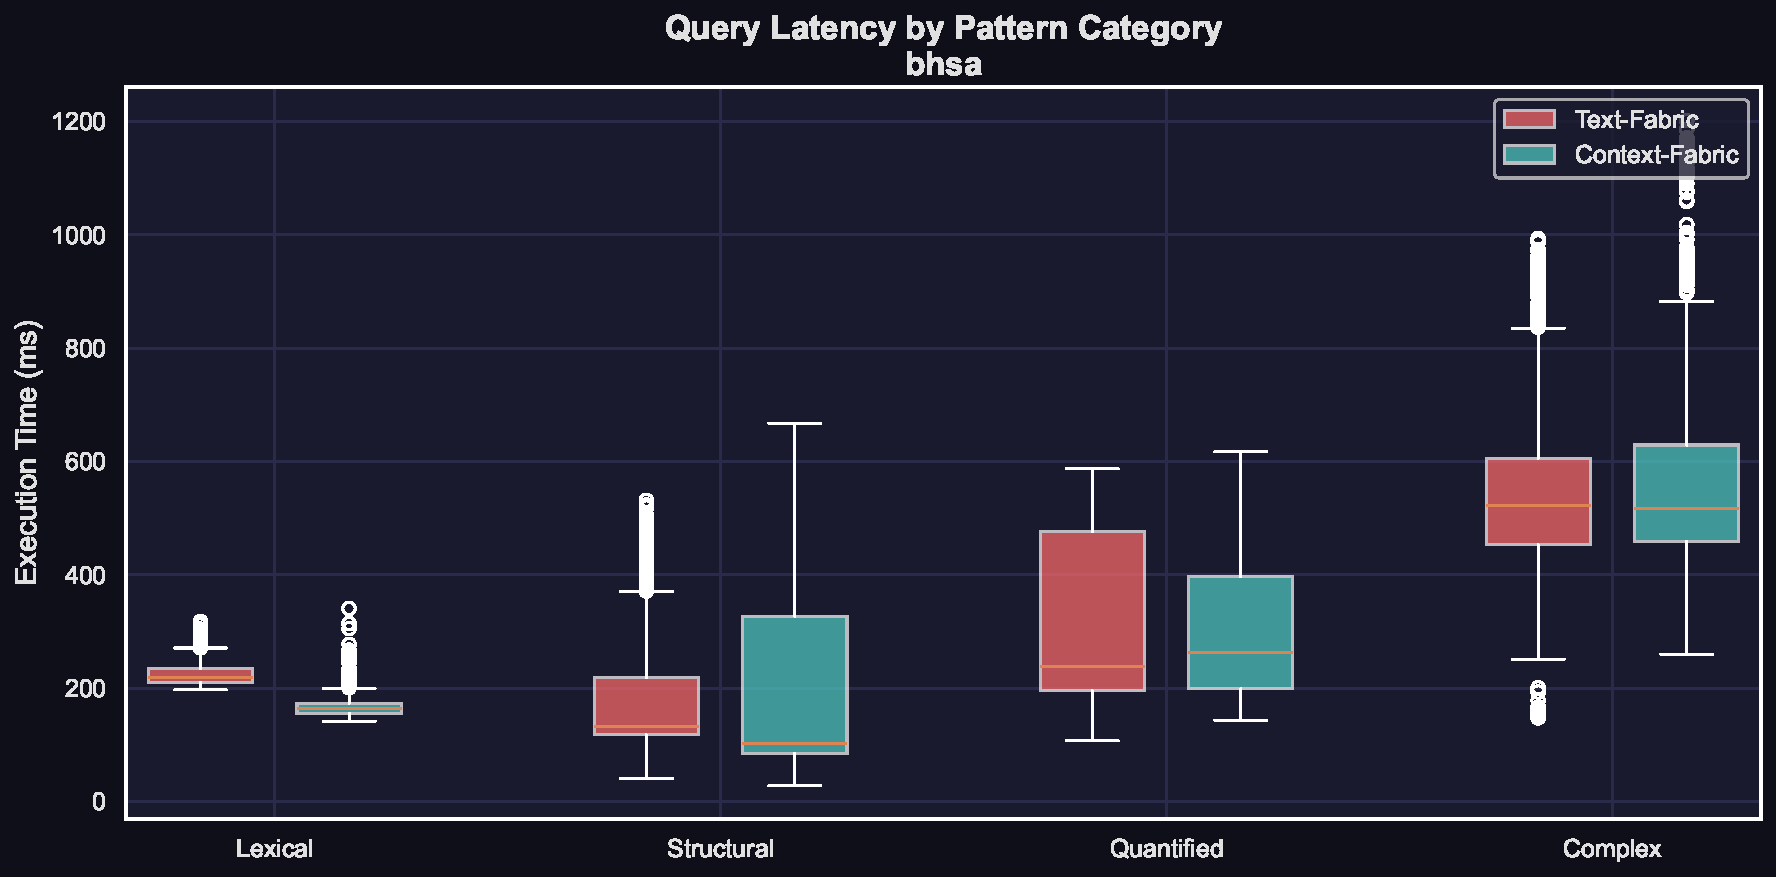
\includegraphics[width=0.9\textwidth]{fig_latency_distribution.pdf}
\caption{Query latency distribution by category. Boxes show interquartile range; whiskers extend to 1.5$\times$ IQR.}
\label{fig:latency_distribution}
\end{figure}

Figure~\ref{fig:latency_percentiles} shows the cumulative distribution of query latencies across all 100 queries. At the median (p50), both implementations perform similarly. At the 95th percentile, TF shows higher latency on lexical queries while CF shows higher latency on complex structural queries. This tradeoff reflects fundamental architectural differences: Text-Fabric's in-memory Python objects enable fast pointer traversal for structural queries, while Context-Fabric's memory-mapped arrays require additional indirection for hierarchical navigation.

\begin{figure}[htbp]
\centering
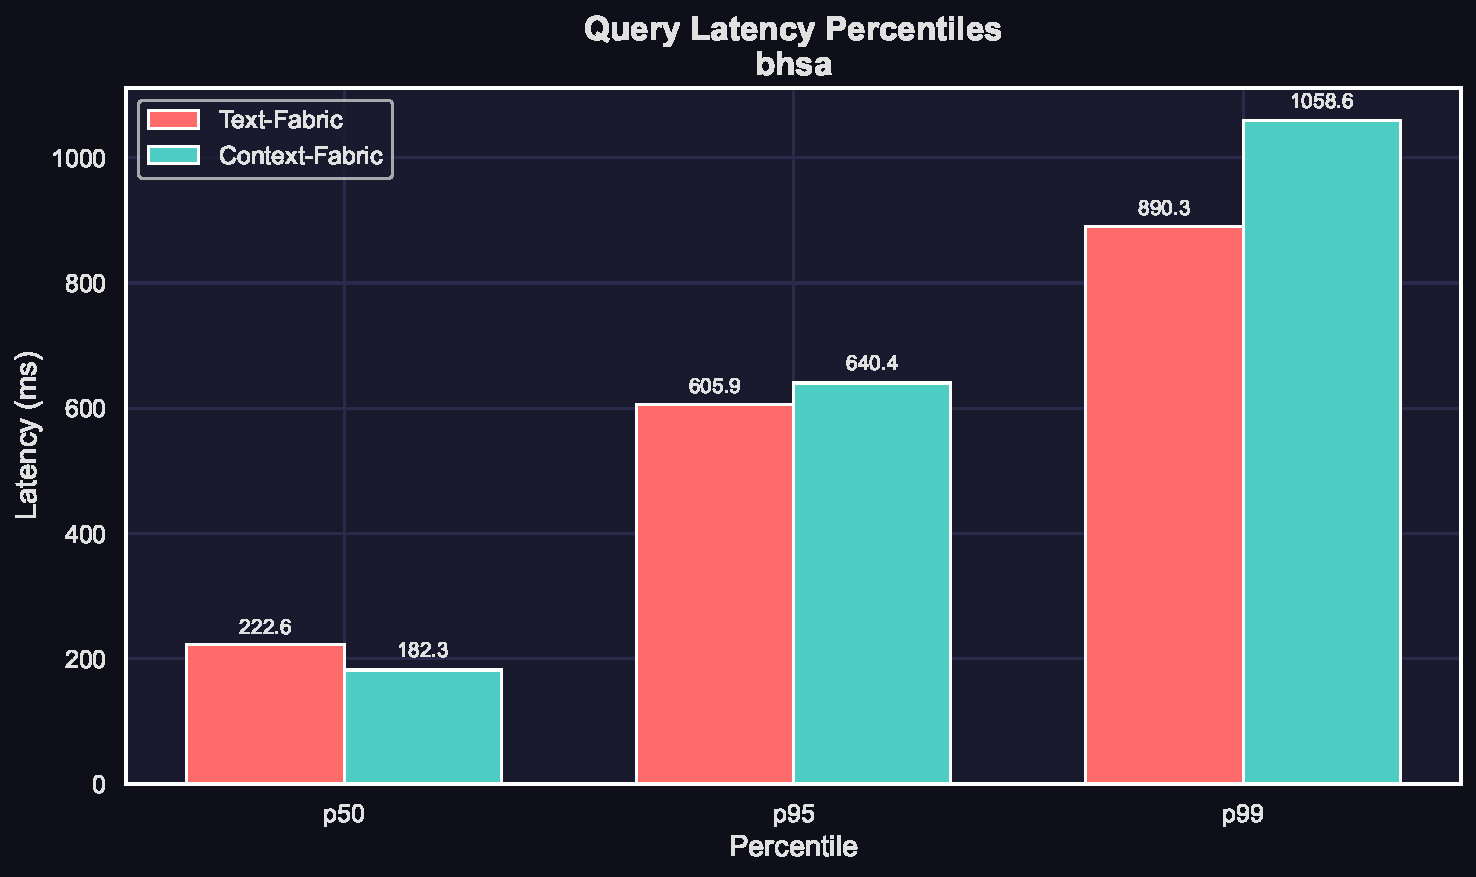
\includegraphics[width=0.9\textwidth]{fig_latency_percentiles.pdf}
\caption{Query latency percentiles (p50, p95, p99) across all 100 benchmark queries.}
\label{fig:latency_percentiles}
\end{figure}

Overall, Context-Fabric achieves a 3\% speedup across all queries while maintaining the dramatic memory advantages documented above. For workloads dominated by lexical queries (common in corpus linguistics), the speedup reaches 26\%. For workloads requiring extensive structural traversal, users may observe modest latency increases that are typically acceptable given the memory savings.

\subsection{Summary of Results}
\label{sec:results-summary}

Table~\ref{tab:results_summary} consolidates the key findings.

\begin{table}[htbp]
\centering
\caption{Summary of benchmark results comparing Text-Fabric and Context-Fabric.}
\label{tab:results_summary}
\begin{tabular}{lll}
\toprule
\textbf{Metric} & \textbf{Result} & \textbf{Interpretation} \\
\midrule
Single-corpus memory & 65\% reduction (mean) & 20--92\% range by corpus size \\
Multi-corpus scaling & 127 vs 677 MB/corpus & 5.3$\times$ scaling advantage \\
10-corpus deployment & 1,348 vs 5,529 MB & 76\% total reduction \\
Load time (large corpora) & Up to 12.9$\times$ faster & BHSA loads in 0.55s vs 7.1s \\
Lexical query latency & 26\% faster & Memory-mapped index access \\
Structural query latency & 6\% slower & Indirection overhead \\
Overall query latency & 3\% faster & Balanced workload \\
\bottomrule
\end{tabular}
\end{table}

The results demonstrate that Context-Fabric achieves its primary design goal: enabling multi-corpus research within constrained memory environments without sacrificing query performance. The 65\% average memory reduction, combined with 5.3$\times$ better scaling characteristics, makes previously impractical research configurations feasible. A researcher with 16 GB of RAM can now work with corpora that would have required 40+ GB under the traditional architecture.

\section{Populating Agentic Context}

\subsection{Automatic Corpus Description}

\subsection{Search Guide}

\section{Using Context-Fabric}

\subsection{Installation}

Context-Fabric is available on PyPI:

\begin{lstlisting}[language=bash]
pip install context-fabric
\end{lstlisting}

Source code and documentation are available at \url{https://github.com/Context-Fabric/context-fabric}.

\subsection{Reproducibility}

All benchmarks can be reproduced using the \texttt{cfabric-benchmarks} package:

\begin{lstlisting}[language=bash]
# Install and download corpora
pip install cfabric-benchmarks
python -m cfabric_benchmarks.corpora.download

# Run full benchmark suite
cfabric-bench full --corpora-dir .corpora
\end{lstlisting}

Results are saved to \texttt{benchmark\_results/} with timestamps. Configuration, environment metadata, and raw measurements are preserved for reproducibility.

\subsection{Usecases}

\section{Future Direction}

Context-Fabric is being re-written in Rust, which will bring an even further step-change in performance.

% Needs to be updated and audited
\begin{thebibliography}{99}

\bibitem{textfabric}
Roorda, D. (2018). Text-Fabric: Text representation for linguistic annotation. \textit{Research Data Journal for the Humanities and Social Sciences}, 3(1), 1--23.

\bibitem{bhsa}
van Peursen, W. Th., Sikkel, C., \& Roorda, D. (2015). Hebrew Text Database BHSA. DANS. \url{https://doi.org/10.17026/dans-z6y-skyh}. Data curated by the Eep Talstra Centre for Bible and Computer, Vrije Universiteit Amsterdam.

\bibitem{lxx}
Center for Biblical Languages and Computing. (2024). Septuagint (Rahlfs' LXX Edition 1935) in Text-Fabric. Based on Eliran Wong's RLXX1935 dataset. GitHub: \url{https://github.com/CenterBLC/LXX}

\bibitem{n1904}
Center for Biblical Languages and Computing. (2024). Nestle 1904 Greek New Testament in Text-Fabric. GitHub: \url{https://github.com/CenterBLC/N1904}

\bibitem{dss}
Jacobs, J., Naaijer, M., \& Roorda, D. (2017). Dead Sea Scrolls in Text-Fabric. Data provided by Martin Abegg. Developed as part of the CACCHT project. GitHub: \url{https://github.com/ETCBC/dss}

\bibitem{peshitta}
van Peursen, W. Th., Veldman, G. J., Sikkel, C., Vlaardingerbroek, H., \& Roorda, D. (2018). ETCBC/peshitta: Syriac Old Testament (Peshitta) in Text-Fabric. Zenodo. \url{https://doi.org/10.5281/zenodo.1464757}

\bibitem{syrnt}
Vlaardingerbroek, H. \& Roorda, D. (2017). Syriac New Testament in Text-Fabric. Source data from SEDRA database by George A. Kiraz and James W. Bennett. GitHub: \url{https://github.com/ETCBC/syrnt}

\bibitem{sp}
Naaijer, M., Højgaard, C. C., Schorch, S., \& Ehrensv{\"a}rd, M. (2020). Samaritan Pentateuch in Text-Fabric. Developed as part of the CACCHT project. GitHub: \url{https://github.com/DT-UCPH/sp}

\bibitem{tischendorf}
Kingham, C. (2018). Tischendorf 8th Edition Greek New Testament in Text-Fabric. Based on Ulrik Sandborg-Petersen's corpus. GitHub: \url{https://github.com/codykingham/tischendorf_tf}

\bibitem{quran}
van Lit, C. \& Roorda, D. (2017). Quranic Arabic Corpus in Text-Fabric. Source data from the Quranic Arabic Corpus and Tanzil project. GitHub: \url{https://github.com/q-ran/quran}

\bibitem{cuc}
Højgaard, C. C., Naaijer, M., Ehrensv{\"a}rd, M., et al. (2020). Copenhagen Ugaritic Corpus in Text-Fabric. Developed as part of the CACCHT project. GitHub: \url{https://github.com/DT-UCPH/cuc}

\bibitem{wikipediarss}
Wikipedia contributors. (2024). Resident set size. \textit{Wikipedia, The Free Encyclopedia}. Retrieved from \url{https://en.wikipedia.org/wiki/Resident_set_size}

\bibitem{wikipediammap}
Wikipedia contributors. (2024). Memory-mapped file. \textit{Wikipedia, The Free Encyclopedia}. Retrieved from \url{https://en.wikipedia.org/wiki/Memory-mapped_file}

\bibitem{baeldunglinuxmem}
Baeldung. (2024). Understanding memory usage in Linux. \textit{Baeldung on Linux}. Retrieved from \url{https://www.baeldung.com/linux/resident-set-vs-virtual-memory-size}

\bibitem{beyer2019reliable}
Beyer, D., L{\"o}we, S., \& Wendler, P. (2019). Reliable benchmarking: requirements and solutions. \textit{International Journal on Software Tools for Technology Transfer}, 21(1), 1--29.

\bibitem{langner2021mess}
Langner, T., \& Beyer, D. (2021). Mess: Memory consumption benchmarking made easy. \textit{arXiv preprint arXiv:2106.08235}. Retrieved from \url{https://arxiv.org/abs/2106.08235}

\bibitem{sqlitemmap}
SQLite Consortium. (2024). Memory-Mapped I/O. \textit{SQLite Documentation}. Retrieved from \url{https://sqlite.org/mmap.html}

\bibitem{cmummap}
Crotty, A., Leis, V., \& Pavlo, A. (2022). Are You Sure You Want to Use MMAP in Your Database Management System? \textit{Proceedings of the 12th Annual Conference on Innovative Data Systems Research (CIDR)}. Retrieved from \url{https://db.cs.cmu.edu/mmap-cidr2022/}

\bibitem{numpymemmap}
NumPy Developers. (2024). numpy.memmap. \textit{NumPy Documentation}. Retrieved from \url{https://numpy.org/doc/stable/reference/generated/numpy.memmap.html}

\bibitem{ipythonmemmap}
Rossant, C. (2018). Processing large NumPy arrays with memory mapping. \textit{IPython Cookbook, 2nd Edition}. Retrieved from \url{https://ipython-books.github.io/48-processing-large-numpy-arrays-with-memory-mapping/}

\bibitem{colibricore}
van Gompel, M. \& van den Bosch, A. (2016). Efficient n-gram, skipgram and flexgram modelling with Colibri Core. \textit{Journal of Open Research Software}, 4(1), e30. \url{https://doi.org/10.5334/jors.105}

\bibitem{cqpweb}
Hardie, A. (2012). CQPweb---combining power, flexibility and usability in a corpus analysis tool. \textit{International Journal of Corpus Linguistics}, 17(3), 380--409.

\bibitem{sketchengine}
Kilgarriff, A., Baisa, V., Bu\v{s}ta, J., Jakub\'{i}\v{c}ek, M., Kov\'{a}\v{r}, V., Michelfeit, J., Rychl\'{y}, P., \& Suchomel, V. (2014). The Sketch Engine: ten years on. \textit{Lexicography}, 1(1), 7--36.

\end{thebibliography}

\end{document}
